%%%%%%%%%%%%%%%%%%%%%%%%%%%%%% -*- Mode: Latex -*- %%%%%%%%%%%%%%%%%%%%%%%%%%%%
%% 05-01-hackystat.tex -- Thesis - Priority Ranked Inspection
%% Author          : Aaron A. Kagawa
%% Created On      : Mon Sep 23 11:52:28 2004
%% Last Modified By: Aaron Kagawa
%% Last Modified On: Tue Jul  5 20:13:57 2005
%% RCS: $Id$
%%%%%%%%%%%%%%%%%%%%%%%%%%%%%%%%%%%%%%%%%%%%%%%%%%%%%%%%%%%%%%%%%%%%%%%%%%%%%%
%%   Copyright (C) 2004 Aaron A. Kagawa
%%%%%%%%%%%%%%%%%%%%%%%%%%%%%%%%%%%%%%%%%%%%%%%%%%%%%%%%%%%%%%%%%%%%%%%%%%%%%%%

\chapter{The Hackystat System}
\label{chapter:hackystat}

The Priority Ranked Inspection process is a theoretical process that can be
implemented in many different ways. In this research, I utilized the
Hackystat system to implement the PRI process for a specific organization.
This chapter is a brief introduction to the Hackystat system, which was
invented by Professor Philip M. Johnson, in the Collaborative Software
Development Laboratory, Department of Information and Computer Sciences,
University of Hawaii at Manoa.

\section{Overview of the Hackystat System}
The Hackystat system is an open-source software framework for the automated
collection and analysis of software product and process measures. Product
measures can be defined as measures that are obtainable from direct
analysis of source code. For example, some product measures include: lines
of code, dependency, and the number of unit tests. Process measures can be
defined as measures that are obtainable from the actual development
process, which creates the source code. For example, some process measures
include: the number of developers, the developers' ``effort'', the number
of major releases, and the number of defects.

The following list summarizes the features that Hackystat provides
\cite{Johnson05}:

\begin{enumerate}
\item Hackystat utilizes custom ``sensors'' that are ``attached'' to
  various software development tools. Theses sensors unobtrusively collect
  data on various software product and development process measures. 
\item Hackystat supports any and all software projects, development
  processes, software development environments, operating systems, and
  development tools. 
\item Hackystat supports in-process project management by providing a set
  of extendible analyses of the product and process measures that are
  collect by the sensors.
\item Hackystat is well suited for empirical software development
  experimentation.
\end{enumerate}

The Hackystat system is a mature and extendible software system. Currently,
Hackystat is being utilized by NASA's Jet Propulsion Laboratory, Sun
Microsystems, IBM, Ikazyo.org, University of Torino, University of
Maryland, and of course the University of Hawaii. A few of the many
publications associated with Hackystat are the following:
\cite{csdl2-04-22, csdl2-04-13, csdl2-04-11, csdl2-03-12, csdl2-02-07,
  csdl2-03-07, csdl2-04-02, csdl2-04-04, csdl2-04-06}

\section{Hackystat's Architecture}
Figure \ref{fig:hackystat-architecture} presents one way of viewing
Hackystat's architecture. Rather than paraphrase the information provided
in Hackystat's User Guide, I provide the entire segment about Hackystat's
architecture \cite{Johnson05}. 

\begin{quotation}
  \textit{ In this view, the ``clients'' are development environment tools,
    such as editors (Emacs, Eclipse, Vim), configuration management systems
    (CVS, Harvest), build tools (Ant, Make), Unit Testing tools (JUnit),
    and so forth. For each of these tools, a custom Hackystat sensor must
    be developed. It is ``custom'' in the sense that it must use the
    plug-in or extension point API for the tool, and ``custom'' in the
    sense that the type of product or process data that it collects is
    specific to the tool it supports. \newline \newline Once data is
    collected by these client-side sensors, it is transmitted using SOAP to
    the ``server'', which is a custom web application running within a
    conventional servlet-supporting web server such as Apache Tomcat. Note
    that the client-side sensors have the ability to cache data in the
    event that a network connection cannot be made to the server and resend
    it later, allowing the developers to work offline. \newline \newline
    Upon receipt of the ``raw'' sensor data by the server, various analyses
    can be run. Some of these analyses are run automatically by the server
    each day, others are run only when invoked by developers from a Web
    Browser interface. The goal of these analyses are typically to create
    abstractions of the raw sensor data stream that help developers and
    managers to interpret the current state and trajectory of the project
    and gain insight into possible problems or opportunities for
    improvement going forward. \newline \newline In certain cases, these
    abstractions can be automatically emailed back to the developers on a
    daily basis, creating a feedback loop.}
\end{quotation}

\begin{figure*}[h]
  \centering
  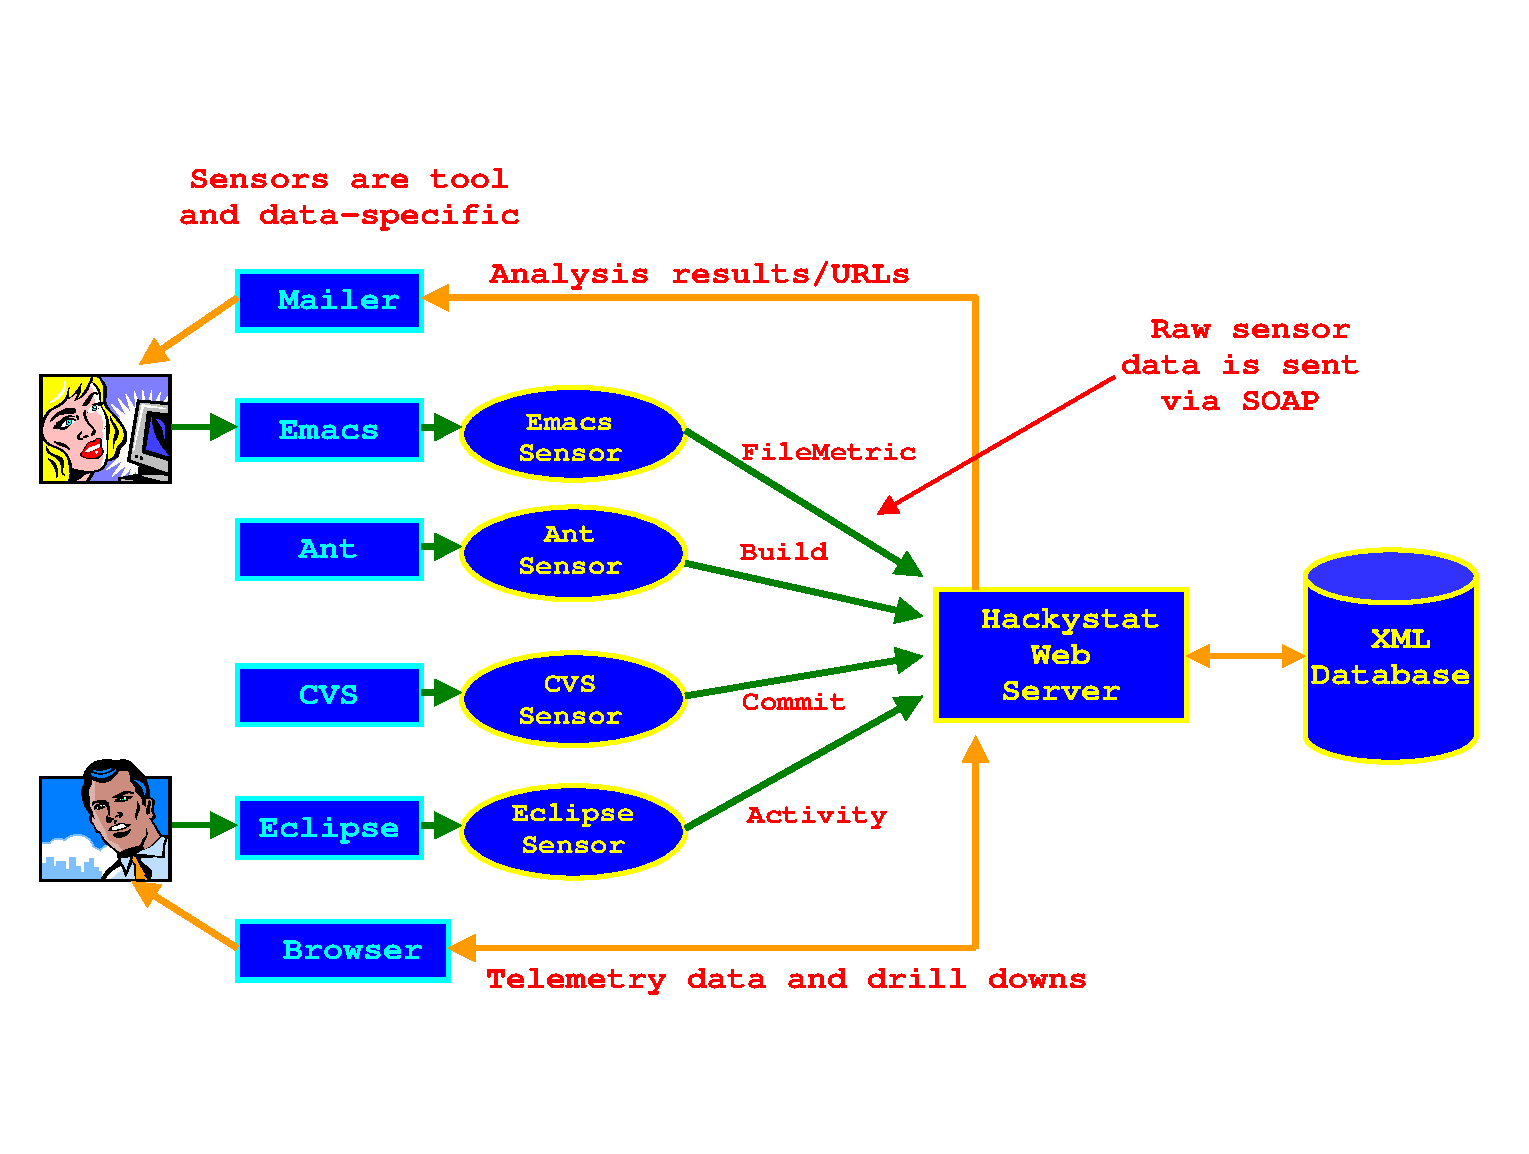
\includegraphics[width=1.00\textwidth]{figs/Architecture.eps}
  \caption[Hackystat Architecture]{Displays a high level overview of the
    Hackystat architecture}
  \label{fig:hackystat-architecture}
\end{figure*}

\section{Hackystat Sensors}
Figure \ref{fig:hackystat-sensors-dataTypes} presents a mapping between
Hackystat's sensors and sensor data types. Once again, rather than
paraphrase the information provided in Hackystat's User Guide, I provide
the entire segment about Sensor Data Types \cite{Johnson05}.

\begin{quotation}
  \textit{ A ``sensor data type'' represents the structure of a single kind
    of software product or process measurement. For example, the
    ``UnitTest'' sensor data type represents the outcome of invoking a
    single unit test. This data typically includes the time that the unit
    test was invoked, the class name of the unit test code, and the results
    of the invocation (pass, fail, exception). The ``Commit'' sensor data
    type represents the occurrence of committing a file to a configuration
    management repository, and thus has very different fields associated
    with it that are appropriate to this kind of event. A given sensor can
    collect data for one or more sensor data types.}
\end{quotation}

\begin{figure*}[h]
  \centering
  \includegraphics[width=1.00\textwidth]{figs/Sensors-DataTypes.eps}
  \caption[Hackystat Sensors and Sensor Data Types]{Displays the
    connections between the Sensors and the Sensor Data Types provided in
    Hackystat.} 
  \label{fig:hackystat-sensors-dataTypes}
\end{figure*}


\section{Some Screenshots of Hackystat}
\begin{figure*}[h]
  \centering
  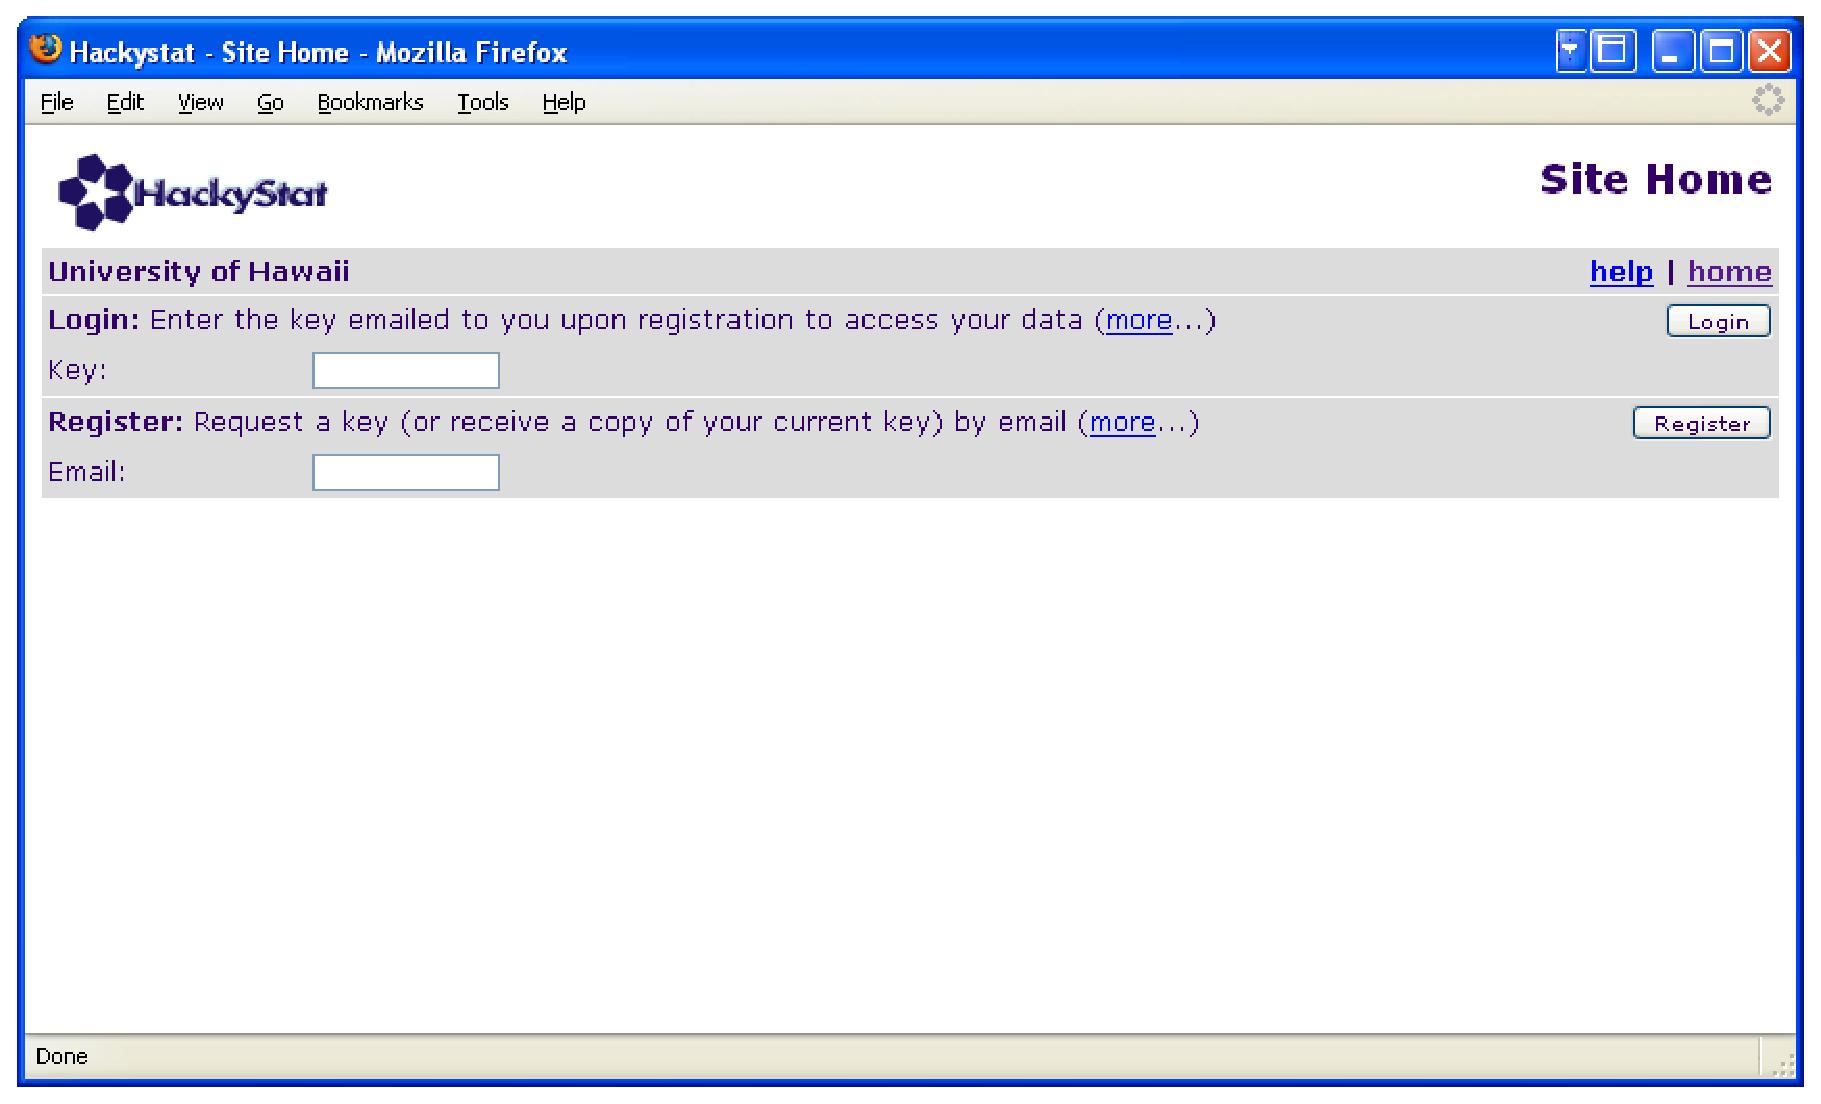
\includegraphics[width=1.00\textwidth]{figs/UserInterface/page-home.eps}
  \caption[The Hackystat Home Page]{Displays the Hackystat home page. 
    Hackystat is designed to protect the data of its users. Therefore, the
    system requires a registration and login before using Hackystat.}
  \label{fig:page-home}
\end{figure*}

\begin{figure*}[htbp]
  \centering
  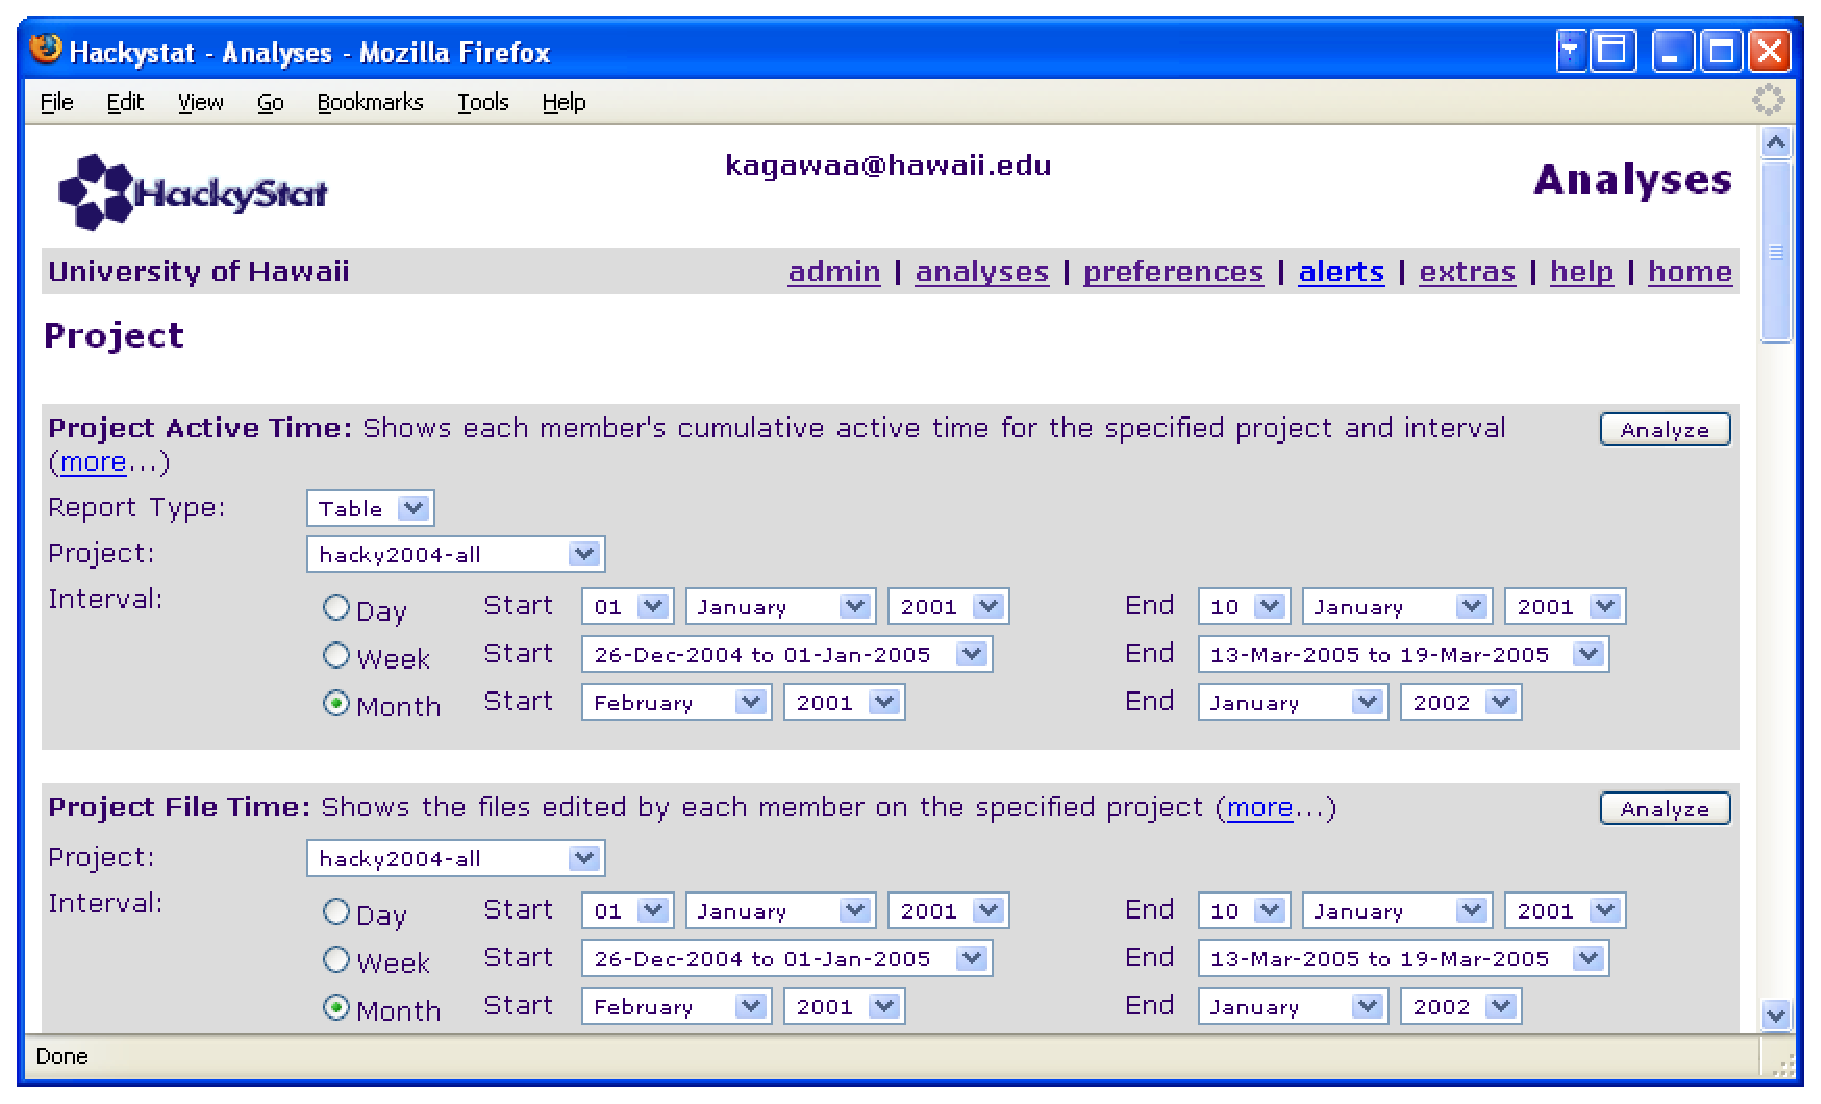
\includegraphics[width=1.00\textwidth]{figs/UserInterface/page-analysis.eps}
  \caption[The Hackystat analysis webpage]{Provides a listing of all
    available Hackystat analyses. Each analysis displays its results with
    image charts, HTML tables, and downloadable files.}
  \label{fig:page-analysis}
\end{figure*}

\begin{figure*}[htbp]
  \centering
  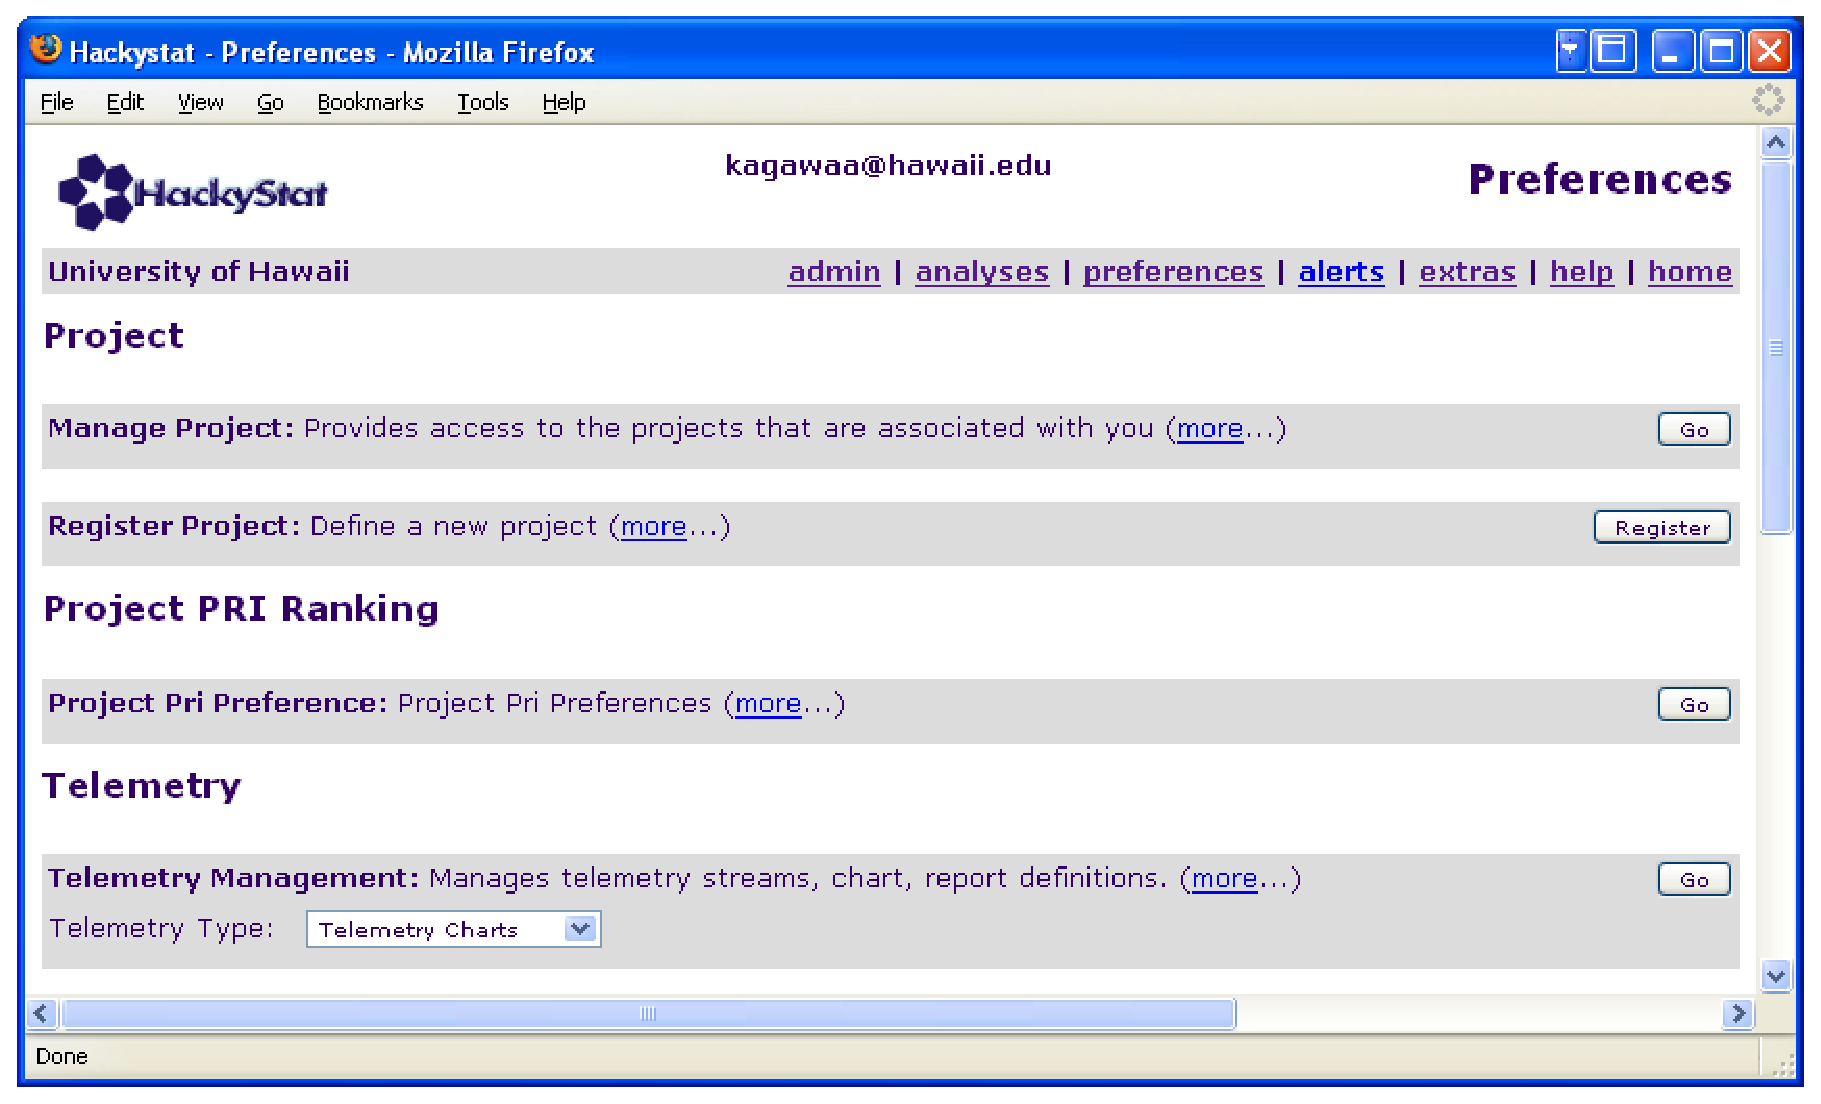
\includegraphics[width=1.00\textwidth]{figs/UserInterface/page-preferences.eps}
  \caption[The Hackystat preferences webpage]{Provides a listing of all
    preferences, which allow users to set specific settings that are
    sometimes required and sometimes optional to run analyses on the
    Hackystat server.}
  \label{fig:page-preferences}
\end{figure*}

\clearpage
\section{More Information about Hackystat}
The Hackystat system can be downloaded for use in other software
organizations by visiting the Hackystat Developer Services website
(http://www.hackystat.org). In addition, Hackystat's User Guide, full
source code, Java documentation, and other useful information that are
required to install Hackystat are obtainable at this website. Any questions
and suggestions can be sent to Hackystat Users email mailing list
(hackystat-users-l@hawaii.edu).









